%\documentclass[a4paper]{article}
%\usepackage[utf8]{inputenc}
%\usepackage[ngerman]{babel}
%\usepackage{amsmath}
%\usepackage{amssymb}
%\usepackage{algorithm2e}
%\usepackage{graphicx}

%\title{\textbf{foo}\\bar }
%\author{Andreas Fuchs, 1106307}
%\date{\today}


%\begin{document}

%\maketitle
%\tableofcontents
%\newpage

%%%
%%%
%%%
\section{Die Objekt Orientierte Ära}

\subsection{Motivation:}

Seit dem Aufkommen von Datenbanksystemen ist es üblich die (persistenten) Daten von der Applikation zu trennen. Dadurch werden persistente Daten, üblicherweise durch ein DBMS verwaltet, anders behandelt als programmeigene Daten die nur während der Laufzeit existieren. Um also auf persistenten Daten zu arbeiten und diese zu manipulieren musste also eine Sprache in die andere eingebunden werden - üblicherweise durch Aufrufe aus der Applikation an das DBMS.

Dies hatte zum einen den Nachteil dass Applikationsentwickler sowohl in der Programmiersprache des Programms als auch in der Abfragesprache des DBMS vertraut sein mussten.

Zusätzlich führte die fortschreitender Entwicklung von Programmierparadigmen und dem Durchbruch Objektorientierter Programmierung (OOP) zu einem sogenannten \emph{impedence mismatch} \cite{copeland1984}. Dies ist wenn sich die Programmiersprache der Applikation und des DBMS auf konzeptioneller und struktureller weiße Unterscheiden und die damit verbunden Schwierigkeit Daten in einer Form in der anderen zu repräsentieren.

Im speziellen können im \emph{Object-Relational Impedance Mismatch} folgende Schwierigkeiten ausgemacht werden \cite{ireland2009}


\begin{description}
	\item \textbf{Struktur:} 
		Eine Klasse besitzt sowohl eine beliebige Struktur die möglicherweise Pointern/Referenzen oder benutzerdefinierten Datentypen enthält als auch beliebige Semantik, definiert durch ihre Methoden. Sie ist möglicherweise auch Teil einer Klassenhierarchie. Ein Tupel besteht nur aus reinen Werten (einfachen Datentypen) und ist kein Teil einer Hierarchie.
	
	\item \textbf{Instanz:}
		Ein Objekt ist eine Instanz einer Klasse. Ein Tupel ist eine Wahrheitsaussage über ein Universum.
	
	\item \textbf{Kapselung:} 
		Der zugriff auf die Daten eines Objekts wird über Methoden geregelt. Keine solche Regelung existiert im Relationalen Modell und Daten können beliebig verändert werden.
	
	\item \textbf{Identität:}
		Jedes Objekt besitzt eine Identität unabhängig ihres Zustands. Ein Tupel ist über ihren Zustand definiert. 
	
	\item \textbf{Arbeitsweise:}
		Ein Objektmodell ist ein Netzwerk interagierender Objekte die über Methoden kommunizieren während das das Relationale Modell als Menge betrachtet werden kann und prozedural abgearbeitet werden.
	
	\item \textbf{Organisatorisch:} 
		Die Besitzer der Applikation und der Datenbank können verschieden sein. Das erschwert es bei Änderungen das Klassenmodell und das Datenbankschema synchron zu halten. 
	
\end{description}


\subsection{Objektorientierte Datenbanksysteme (OODBS)}
Um diese Probleme zu beheben war es naheliegend den Umweg von der Applikation zu den persistenten Daten über ein (externes) DBMS zu ersparen und einen weg zu Entwickeln der es erlaubt die Objekt in der Programmiersprache selbst persistent zu machen. Deswegen werden die OODBS auch oft \emph{Persistente Programmiersprachen} genannt.

\subsubsection{Frühe Ansätze}
Bereits in den späten 1970ern wurde mit ersten Prototypen wie Pascal-R oder Rigel experimentiert. Es dauerte jedoch bis Mitte der 1980er dass verschiedene kommerzielle Anbieter persistente Programmiersprachen am Markt anboten. Diese richteten ihre Aufmerksamkeit meist auf den Technischen und Planerischen Bereich. Aufgrund dieser markttechnischen Ausrichtung lag der Fokus dieser frühen OODBS wenig auf Abfragesprachen und Transaktionsmanagement und mehr auf der Performance. Obwohl einige Umsetzungen Innovative Architekturen boten um dieses Ziel umzusetzen fanden persistente Programmiersprachen nur geringe Verbreitung vornehmlich bei CAD-Anwendungen.

%competitive in performance with conventional method (programmiersprache + load programm) zB Programmperformance ggf um einiges schlechter falls bei jeder änderung auf platte geschrieben wird 

Grund für das Scheitern waren das fehlen von Standards und die Abhängigkeit von der eingesetzten Programmiersprache. Applikationen die nicht in der selben Programmiersprache geschrieben sind haben auch keinen Zugriff auf die persistenten Daten. Für die Kunden schien der Vorteil keine Schnittstelle Entwickeln zu müssen als zu geringer Gewinn \cite{stonebraker} um die Nachteile aufzuwiegen.

Um einige der Nachteile zu beseitigen schickte sich die \emph{Object Database Management Group} (ODMG), ein Zusammenschluss verschiedener Objektorienter Datenbanksystemanbieter, in den 90ern dazu an einen Standard für Objetorientierte Datenbanksysteme inklusive einer an SQL angelehnten Abfragesprache \emph{Object Query Language} zu etablieren. Im Jahr 2000 erschien der Standard 3.0 woraufhin die ODMG als ihr Ziel als erreicht ansah und sich 2001 auflöste \cite{http://www.odbms.org/odmg-standard/}.

Dennoch haben bis heute OODBS nur eine geringe Verbreitung.


\subsubsection{Schwierigkeiten}
Einer der größten Hindernisse eine Programmiersprache mit DBMS Funktionalität zu erweitern ist, dass die Compiler mit dieser Funktionalität erweitert werden müssen. Dies betrifft nicht nur Compiler verschiedener Sprachen, aber auch Compiler derselben Sprache. Zum Beispiel sollte C++ mit DBMS Funktionalität erweitert werden müssen Compiler wie GCC oder Intel C++ Compiler jeweils dies Unterstützen. Eine solche Unterstützung hat sich bis heute nicht durchgesetzt und die Persistenz muss mit anderen Mitteln - zum Beispiel durch Typbibliotheken wie es die ODMG vorsieht - bereitgestellt werden.

Ein weitere nicht zu unterschätzende Schwierigkeit stellt die Komplexität von Programmiersprachen dar. Aufgrund dieser Komplexität ist es einfach das Programmfehler entstehen die die Datenbestände ungewollt manipulieren. In einer Welt in der Daten oft einen hohen unternehmerischen Wert darstellen ist dies ein deutliches Hindernis. 


\subsection{Objektrelationale Abbildung}
Ein Ansatz den Impedance Missmatch zu umgehen ist, die Abbildung von dem Objetkorientierten auf das Relationale Modell dem Entwickler aus der Hand zu nehmen und durch ein Framework zu automatisieren. Dies löst zwar nicht direkt den impedance mismatch, diese ist jedoch für den Softwareentwickler im idealen Fall nicht mehr sichtbar.

Versuche einer Objektrelationealen Abbildung (ORA) gehen zurück bis auf 1984 \cite{ireland2009}, es dauerte jedoch bis in die 90er - zum teil vorangetrieben durch den geringen Fortschritt in OODBS - bis erste Produkte wie \emph{TopLink} auf dem Markt erschienen. Seitem haben sich eine Vielzahl an Produkten für verschiedene Programmiersprachen wie zum Beispiel Hibernate für Java oder das Entity Framework für .NET etabliert. 


\subsubsection{Schwierigkeiten}
Entgegen der Häufigen Annahme kann Objektrelationale Abbildung die Abbildung von der objektorientierten auf das relationale Modell nicht vollständig automatisieren. 

Auch wenn Objektrelationale Abbildungen ein hilfreiches Werkzeug für den Entwickler sein können, ist die Verwendung solcher weder trivial noch vollständig automatisiert. Die Verwendung von ORA ohne die Auswirkungen auf die Datenbankperformance zu berücksichtigen kann zu Performance Antipattern führen die langsame Reaktionszeiten oder gar den Stillstand eines System verursachen können \cite{chen2014}.

Erschwerend kommt hinzu dass für die verschiedenen ORAs keine einheitlich Standards festgelegt sind. So können gleiche oder ähnliche Konzepte in den verschiedenen ORAs unterschiedlich benannt sein und sie können sich sehr in ihrer Funktionalität unterscheiden \cite{torres2017}.


\subsection{Beispiel ODMG C++}
\label{oo-example-section}
Angenommen wir haben eine Klasse Person mit den Attributen Name und Adresse sowie eine von der Person abgeleitet Klasse Student mit dem zusätzlichen Attribut matrikelnummer. Es existiert noch eine weitere Klasse Universität und jeder Student ist auf einer Universität eingeschreiben welches durch eine Refernz auf Universität abgebildet wird, siehe Abbildung \ref{oo-example}

\begin{figure}[htp]
\centering
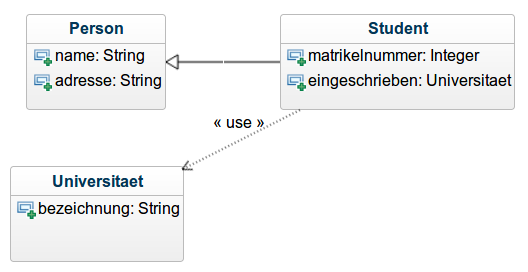
\includegraphics[width=0.7\textwidth]{images/OODBS-class-diagram.png}
\caption{Beispiel Objekt Orientierung}
\label{oo-example}
\end{figure}

Für die Klasse die Persistent werden soll muss die ODMG-Klasse d\_Object als Superklasse eingebunden werden. Wie Üblich wird diese Eigenschaft an die abgeleiteten Klassen vererbt, es ist also nicht nötig die Klasse d\_Object noch einmal einzubinden. Die Persistenz wird dabei während der Erzeugung deklariert. Objekte können andere Objekte über einen smart pointer \emph{d\_Ref} referenzieren. Alle primitiven C++ Datentypen bis auf union, bit fields und references werden explizit unterstützt und einige strukturierte Literale wie zum Beispiel String sowie Collection Typen wie Arrays werden ebenso unterstützt. Algorithm \ref{odl} zeigt unser Beispiel und wie dieses in C++ mit der Object Definition Language (ODL) persistent gemacht werden könnte \ref{vassilis2000}, \ref{kemper2013}.

\vspace{.3cm}
\begin{algorithm}[H]
	% \KwData{this text}
	% \KwResult{how to write algorithm with \LaTeX2e }
	class Person : public d\_Object \{ \\
		%\Indp : shift indentation to right
		%\Indm : shift indentation to left
		\Indp
		d\_String name; \\
		d\_String adresse; \\
		\Indm
	\}

	class Student : Person \{ \\
		%\Indp : shift indentation to right
		%\Indm : shift indentation to left
		\Indp
		d\_Long matrikelnummer;  ~~~// d\_Long ist äquivalent zu unsigned integer \\
		d\_Ref\(<\)Universitaet\(>\) eingeschrieben; \\
%		d\_Rel\_Set ???
%		d\_Set\(<\)d\_Ref\(<\)Universitaet\(>>\) bestuchtLV; \\
		\Indm
	\}

	class Universitaet : public d\_Object \{
		\Indp
		d\_String bezeichnung; \\
		\Indm
	\}
	\caption{C++ Object Definition Language}
	\label{odl}
\end{algorithm}
\vspace{.3cm}

Die Object Query Language (OQL) erlaubt den Zugriff auf die Daten in einer OODBS und ist syntaktisch an SQL angelehnt, bietet jedoch im Vergleich zu SQL:1992 den Vorteil dass man flexibler auf belieb strukturierten Objekten arbeiten kann \cite{kemper2013}. Algorithm \ref{oql} zeigt eine einfache OQL abfrage.

\vspace{.3cm}
\begin{algorithm}[H]
	SELECT s.name \\
	FROM s IN studenten \\
	WHERE universitaet = "{}Uni Wien"{};
	\caption{Object Query Language}
	\label{oql}	
\end{algorithm}
\vspace{.3cm}

%TODO Beispiel OML C++ 

%TODO Beispiel Hibernate?

%\subsection{Object Relational Mapping mit Hibernate}
%Wir verwenden hier wieder das obige Beispiel.

\subsection{Nachwirkungen}
Mit der divergierenden Entwicklung von Programmierparadigmen und Datenbanksystemen, im besonderen die Objektorientierte Programmierung und das Relationale Schema, kam es zu einem deutlichen \emph{Impedance Missmatch}. 
OODBS machten sich daran dieses Problem zu beheben. Trotz der Anstrengungen konnten sich diese jedoch nicht am Markt durchsetzen der nach wie vor vom Relationalen Datenbanken dominiert wird. Zum einen scheinen die Vorteile als zu gering, zum anderen liegt ihr Fokus weniger auf Geschäftsdaten die jedoch eine mächtige Rolle am Markt spielen.
Da die Entwicklung von OODBS in den letzten Jahren stagnierte machte wurde sich zunehmend an die Objektrelationale Abbildung gewandt um das Impedance Mismatch zu beheben. Zwar sind auch diese frei von Problemen und Kritik, dennoch freuen sie sich einer derzeit hohen Verbreitung.


%%%%%%%%
\section{Objektrelationale Datenbanken}
%%%%%%%%

Frühe Relationale Systeme wie INGRES waren hauptsächliche an Geschäftsdaten interessiert und boten nur sehr einfache aber dem Markt entsprechende Datentypen wie Ganzzahlen, Gleitkommazahlen oder Strings sowie nur einfache Operationen. Weiters unterstützten sie nur B-Bäume um in einer Relation zu suchen.

Dies ist jedoch nicht für jeden Markt ausreichend. Geographic Information Systems (GIS) ist ein solcher Markt. In GIS sind Koordinaten als Längen- und Breitengrad angegeben. Eine Koordinate zu finden erfordert somit eine zweidimensionale suche. Ein B-Baum ist jedoch nur in der Lage über eine Dimension zu suchen und ist wenig effizient im Vergleich zu auf mehrdimensionale Suche ausgelegte Bäume wie kd-Trees. Schwieriger noch gestaltet sich eine Suche auf eine Fläche für die es in INGRES keine adäquate Operation gibt da diese von eindimensionalen Daten ausgeht \cite{stonebraker2005}.

Da jeder Markt eigene Anforderungen stellt ist es wenig zielführend die angeforderten Datentypen und Operationen fest zu codieren - ausgenommen der Hersteller beabsichtigt eine Spezialisierung auf diesen Markt. Anstelle sollte es möglich sein dass Kunden die Datenbank möglichst flexibel selbst an ihre Bedürfnisse anpassen können.


\subsection{Objektrelationale Datenbanksysteme}
Dieses Ausgangslage ist der der OODBS nicht unähnlich da hier wie dort sich um einen Impedance Mismatch handelt. Objektrelationale Datenbanksysteme (ORDBS) sind jedoch im Gegensatz zum "{}revolutionären"{} OODBS Ansatz ein "{}evolutionärer"{} Ansatz der versucht das Relationale Modell um die folgenden Eigenschaften zu erweitern \cite{kemper2013}:
\begin{itemize}
	\item \textbf{Große Objekte (Large Objects):} Datentypen die es erlauben auch sehr große Attributwerte zu speichern. Eigentlich handelt es sich hier nur um "{}reine"{} Werte aber dennoch werden sie vielfach den Objektrelationalen Datenbanken hinzugerechnet.
	\item \textbf{Mengenwertige Attribute:} Erlaubt es einem Attribut einen Menge von Werten zuzuordnen.
	\item \textbf{Geschachtelte Relationen:} Erlaubt Attribute die selbst wieder Relationen sind.
	\item \textbf{Typdeklaration:} Erlaubt es dem Benutzer Anwendungsspezifische Typen anzulegen die dann als Attributtypen verwendet werden können. Dies erlaubt komplexe Objektstrukturen.
	\item \textbf{Referenzen:} Attribute können direkte Referenzen auf Tupel beziehungsweise Objekte derselben oder einer fremden Relation sein. Somit ist man nicht mehr nur auf die Verwendung eines Fremdschlüssels beschränkt.
	\item \textbf{Objektidentität} Tupel können eindeutig identifiziert werden und besitzen eine Identität unabhängig ihres Zustands. 
	\item \textbf{Pfadausdrücke:} Referenzattribute machen es erforderlich Pfadausdrücke in der Anfragesprache zu unterstützen
	\item \textbf{Vererbung:} Erlaubt es Generalisierungen beziehungsweise Spezialisierungen umzusetzen.
	\item \textbf{Benutzerdefinierte Operationen:} Erlaubt es den Daten auch eigene Operationen zuzuordnen.
\end{itemize}

\subsubsection{Frühe Ansätze}
Postgres war eine der ersten größeren Objektrelationalen Datenbankdesigns. Es gab auch schon zuvor Versuche die rein Relationale Datenbank INGRES zu erweitern welche jedoch eher in einer Zerstückelung des ursprünglichen INGRES-Designs resultierte. Postgres bot in ihrem ursprünglichen Design im Vergleich eine unter anderem verbesserte Unterstützung komplexer Datentypen sowie die Möglichkeit Benutzerdefinierter Datentypen, Operationen und Methoden ohne jedoch vom Ursprünglichen Relationalen Design abzuweichen um die Kompatibilität zu wahren \cite{stonebraker1986}. Später kamen noch Vererbung, Referenzen und Mengen hinzu \cite{stonebraker1990}. 

Manch andere Datenbanksysteme wie Sybase hatten benutzerdefinierte Funktionen in der Form von \emph{Stored Procedures} ermöglicht welche den Vorteil boten die Anzahl an Transaktionen zu minimieren.

\subsection{Schwierigkeiten}
So wie auch OODBS hatte auch der Objektrelationale Ansatz das Problem dass sich zunächst keine Standards durchgesetzt haben. Dies ist auch heutzutage noch wahr obwohl der SQL:1999 einen Standard verabschiedet hätte, den aber viele Datenbankanbieter noch nicht realisiert haben oder nicht einhalten und stattdessen eigen Methoden bieten.

Eine weitere Ursache die den Durchbruch verzögerte war dass, ebenso wie bei OODBS, es mit zusätzlichen Features auch zu zusätzlicher Komplexität, sowohl für den Hersteller als auch für den Benutzer, kommt. Der Hersteller muss nicht nur die Funktionalität bereitstellen sondern sie soll auch möglichst Performant sein und Abfragen optimieren können. \cite{carey1997} fand dass manche Abfragen, insbesondere jene die Mengen involvieren, auf Objektrelationalen Datenbank weniger Performant sind als jene die dieses Verhalten auf Relationalen Datenbanken simulieren.
Aber auch für den Applikationsentwickler ist die Zunahme an Optionen weniger überschaubar. Insbesondere werden viele der Features kaum verwendet und ein großer Teil der Anwendungsentwickler verwendet die üblichen Features der Relationalen Datenbank und bildet diese auf Applikationsebene auf das objektorientierte Struktur ab. Dies gilt sogar für Objektrelationale Abbildung \cite{fotache2009}.
%TODO: noch etwas ausführlicher aus Paper 470373 oder die zwei Papers in Downloads

\subsection{Beispiel SQL:1999}
Wir Verwenden das selbe Beispiel wie in Abschnitt \ref{oo-example-section} und wollen diese nun auf einen Objektrelationale Datenbank nach dem SQL:1999 Standard abbilden.  Mittels CREATE TYPE kann ein benutzerdefinierter Typ (User Defined Type UDT) angelegt werden. Diese kann auch von einer Oberklasse erben indem mit dem Schlüsselwort UNDER die Oberklasse angegeben wird \cite{gulutzan1999}. Die UDT kann auch Methoden enthalten und es können andere UDTs referenziert werden. Algorithm \ref{sql1999example} zeigt 

\vspace{.3cm}
\begin{algorithm}[H]
	CREATE TYPE person AS \\
	\Indp
		(name varchar(30), adresse varchar(50)); \\
	\Indm 
	~ \\
	CREATE TYPE universitaet AS \\
	\Indp
		(bezeichnung varchar(20)) \\
		METHOD anzahl\_studierende( ) RETURNS int;   \\ \Indp -{}-Methode die später definiert wird \\ \Indm
	\Indm
	~ \\
	CREATE TYPE student UNDER person AS \\
	\Indp
		(matrikelnummer int, \\
		eingeschrieben REF(universitaet)) ~~~-{}- Referenz auf universitaet \\
	\Indm
	\caption{Abbildung Klassen mit SQL:1999}
	\label{sql1999example}
\end{algorithm}
\vspace{.3cm}

\subsection{Nachwirkungen}
Aufgrund des evolutionären Ansatzes des Objektrelationalen Designs fand es einen höheren Anklang als der revolutionäre Ansatz der Obejktorientierten Datenbanksysteme. Das Postgres Design wurde später Implementiert und ständig erweitert und ist heutzutage unter dem Namen PostgreSQL weit verbreitet. 

Der SQL:1999 Standard hatte das Ziel einen standardisiertes Objekt-Relationales Datenmodell einschließlich Anfragesprache zu definieren. Viele dieser Standards sind jedoch bisher von den Datenbanksystemanbietern nicht oder nicht dem Standard entsprechend umgesetzt \cite{kemper2013}. Zumindest bieten aber alle großen Anbieter Relationaler Datenbanken manche Features des Objektrelationalen Designs, wie zum Beispiel stored procedures, in ihren Produkten an.


%\end{document}
